\defi{14.1} Un paralelogramo $\square PABC$ se llama \textbf{rectángulo} si $r_{PA} \perp r_{PC}$


\obs{14.3} Un sistema de \textbf{coordenadas cartesianas} es un par de rectas $l^1$, $l^2 \subset \P$ cortándose ortogonalmente en un punto $O$, llamado \textbf{origen}, siendo así $l^1,l^2$ los \textbf{ejes} [El sistema es construible porque el \tma{2.29} garantiza la existencia de $l_2 \perp l_1$ único pasando por $O$].
Por el \axioma{P3} existen aplicaciones
$$\gamma_k: l^k \rightarrow \R, \;\; k = 1,2$$
tales que 
$$X,Y \in l^k \rightarrow d(X,Y) = \abs{\gamma_k(X) - \gamma_k(Y)}$$
Además, podemos elegir puntos $E^k$ tales que $\gamma_k(O) = 0\;\text{y}\; \gamma_k(E^k)=1$.
Este sistema de coordenadas $OE^1E^2$ es orientado, y a todo punto $A \in \P$ se le pueden asociar dos reales $a_1, a_2$ tales que cada $a^k$ es ortogonal a $l^k$, de modo que $a_k = \gamma_k(A^k)$; y se puede determinar la aplicación de coordenadas $\Gamma(A) = (a_1,a_2)$.



\obs{[Coordenadas en $\E$]} Un sistema de coordenadas en el espacio $\E$ es una terna de rectas $l^1,l^2,l^3$ ortogonales entre sí, los ejes, con un origen $O$; los puntos $E^k$ tales que $d(O, E^k) = 1$ que generan el sistema de coordenadas $OE^1E^2E^3$, y las aplicaciones $\gamma_k$ y $\Gamma$ similares a las de la $\obs{14.3}$ pero con una dimensión más. 

\tma{14.4/14.6/14.7} La aplicación $\Gamma:\P\rightarrow \R^2$ es biyectiva. Si $A,B$ son dos puntos, y $\Gamma(A) = (a_1,a_2)\;;\;\Gamma(B) = (b_1,b_2)$, entonces 
$$d(A,B)^2 = (a_1-b_1)^2+(a_2-b_2)^2$$
Para $\E$, $\Gamma:\E\rightarrow \R^3$ también es biyectiva, y la distancia entre $A, B$ viene dada por 
$$d(A,B)^2 = (a_1-b_1)^2+(a_2-b_2)^2+(a_3-b_3)^2$$

\cor{14.5}/\obs{14.8} El espacio métrico $(\P,d)$ es isométrico a $(\R^2,d_E)$ y $\Gamma:\P\rightarrow\R^2$ es una isometría. El espacio métrico $(\E,d)$ es isométrico a $(\R^3,d_E)$ y $\Gamma:\E\rightarrow\R^3$ es una isometría.

\defi{[Espacio Euclidiano $\R^n$]} El espacio $\R^n$ es el conjunto $\R^n = \{X=(x_1, \cdots, x_n) \; | \; x_i \in \R;\; i = 1,\cdots, n \}$. El conjunto tiene una estructura de \textbf{espacio vectorial} con las operaciones
\[X+Y \equiv (x_1+y_1,\cdots, x_n+y_n) \;;\; X,Y \in \R^n \]
\[\lambda X = (\lambda x_1, \cdots, \lambda x_n) \;;\; \lambda \in \R \]

\defi{14.9 [Distancia euclidiana en $\R^n$]} Para dos puntos $X,Y \in \R^n$ la métrica euclidiana es la aplicación  $d: \R^n \times \R^n \rightarrow \R^+$ tal que
$$d(X,Y) \equiv \left(\sum_{i = 1}^{n}(x_i-y_i)^2\right) ^{1/2}$$

\defi{14.10} El \textbf{producto escalar} de $X,Y$ es
$$\prodvec{X,Y} = X\cdot Y \equiv \sum_{i = 1}^nx_iy_i$$
La \textbf{norma} es la operación 
$$||X||\equiv \langle X,X \rangle^{1/2} = \sum_{i = 1}^nx_i^2$$

\tma{14.11} Para $X,X',Y,Y' \in \R^n$ y $\lambda \in \R$:
\begin{itemizex}
	\item $\prodvec{X,X} \ge 0 \; ;\; \prodvec{X,X} = 0 \iff X = 0$
	\item $\prodvec{X,Y} = \prodvec{Y,X}$
	\item $\prodvec{\lambda X, Y} = \lambda \prodvec{X,Y} = \prodvec{X, \lambda Y}$
	\item $\prodvec{X+X' , Y} = \prodvec{X,Y}+\prodvec{X',Y}\;;\;
	\prodvec{X , Y+Y'} = \prodvec{X,Y}+\prodvec{X,Y'}$
\end{itemizex}

\obs{14.12} El producto escalar y la distancia están relacionados:
\begin{itemizex}
	\item $d(X,Y) = ||X-Y|| = \sqrt{\prodvec{X-Y,X-Y}}$
	\item $d(X,-Y) = ||X+Y||$
	\item $\prodvec{ X, Y} = \frac{1}{4}(||X+Y||^2 - ||X-Y||^2)$
	\item $\prodvec{X, Y} = \frac{1}{2}(||X||^2 + ||Y||^2 - ||X-Y||^2)$
\end{itemizex}

\tma{14.13}  Sea $V \in \R^n\;, \;V \neq 0$. Para todo $U \in \R^n$ existe un único $\lambda_U \in \R$ y un único $V_{U}^\perp$ tales que
$$U = \lambda_UV + V_{U}^\perp\;;\; \prodvec{V, V_{U}^\perp} = 0$$
Además, $\lambda_U$ y $V_U^\perp$ se expresan como
$$\lambda_U= \frac{\prodvec{U,V}}{||V||^2} = \frac{\prodvec{U,V}}{\prodvec{V,V}}\;;\; V_U^\perp = U - \lambda_UV$$
\dem{Por la definición de $U$ tenemos que $\prodvec{U,V} = \prodvec{\lambda_UV+V_U^\perp,V} = \lambda_U\prodvec{V,V}+\cancel{\prodvec{V_U^\perp,V}}\iff\lambda_U= \frac{\prodvec{U,V}}{||V||^2}$\linebreak
	Por otra parte, $\prodvec{V_U^\perp, V} = \prodvec{U-\lambda_UV,V} = \prodvec{U,V} - \lambda_U\prodvec{V,V}= \prodvec{U,V} - \prodvec{U,V}\frac{||V||^2}{||V||^2} = 0$}
\begin{figure}[H]
	\centering
	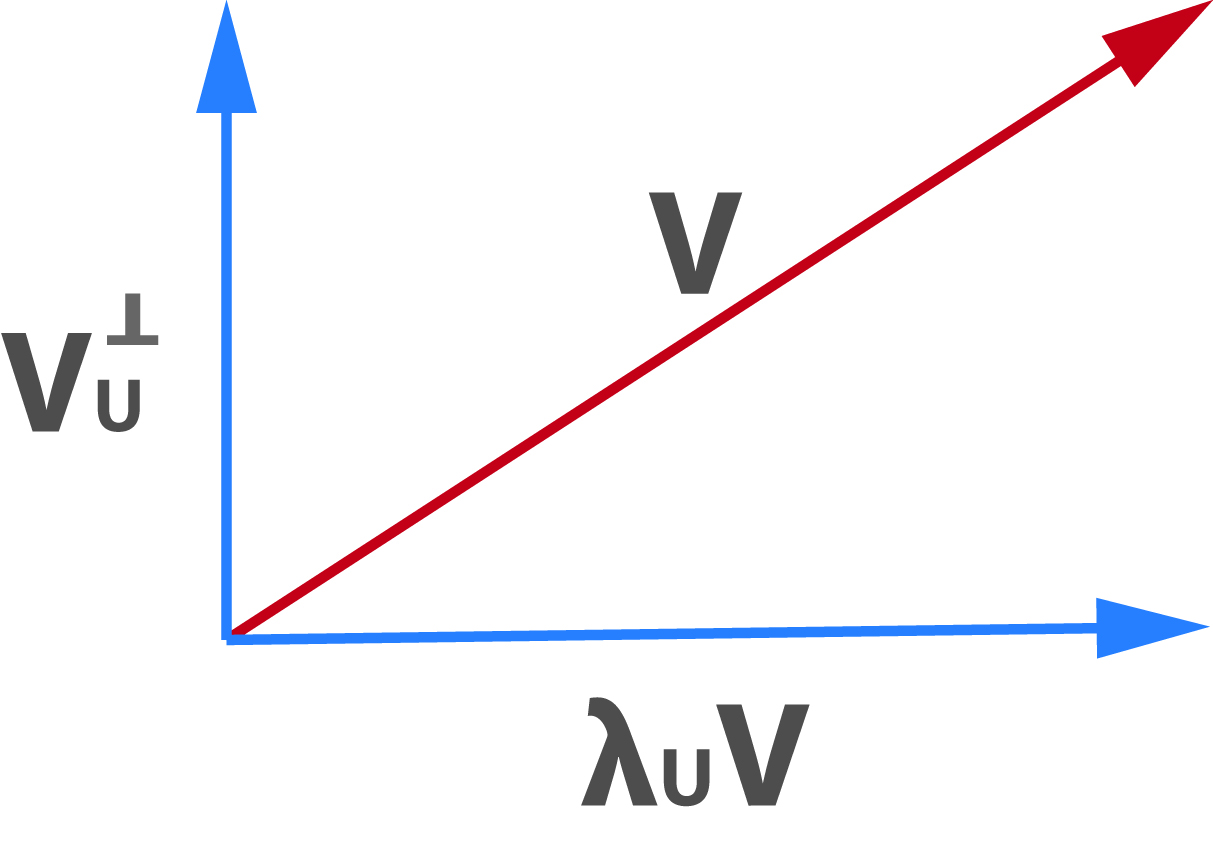
\includegraphics[width=5.5cm]{figuras/13-13.jpg}
	\vspace{-1em}
\end{figure}
\tma{14.14} $(\R^n,d)$ es un espacio métrico: para cada terna $X,Y,Z\in\R^n$ se satisface
\begin{itemizex}
	\item $d(X,Y) \ge 0\;;\; d(X,Y) = 0 \iff X=Y$
	\item $d(X,Y) = d(Y,X)$
	\item $d(X,Z) + d(Z,Y) \ge d(X,Y)$
\end{itemizex}
\dem{Para la tercera afirmación: $V = Y-X$. Segun 14.13, existen $\lambda, W$ tales que $Z-X = \lambda V+W\;;\;\prodvec{V,W} = 0$. Si $Z-Y = Z-X-(Y-X) = (\lambda-1)V+W$ y manipulamos las distancias:
$$||Z-X||^2 = \prodvec{\lambda V+W,\lambda V+W} = \lambda^2||V||^2 + ||W||^2$$
$$||Z-Y||^2 = \prodvec{(\lambda-1)V + W, (\lambda - 1)V + W} = (\lambda - 1)^2||V||^2 + ||W||^2 $$
Y, por tanto
$$||Z-X||+||Z-Y|| \ge |\lambda|\cdot||V|| + |\lambda-1|\cdot||V|| \ge ||V|| = ||Y-X||$$}
\obs{14.15} Para $A,B \in \R^n$ se llama \textbf{segmento de recta}, $[A,B]$ al conjunto
$$[A,B] = \{X \in \R^n \;|\; d(A,X) + d(X,B) = d(A,B) \}$$
o, empleando el \tma{14.14}
$$[A,B] = \{Z \in \R^n\;|\; Z = A + \lambda(B-A)\;,\; \lambda\in [0,1]\}$$

\ej{14.2 [Desigualdad de Cauchy-Schwarz]} Sean $U,V \in \R^n,\; V\neq 0$. Entonces
$$\prodvec{U,V}^2 \le ||U||^2\cdot||V||^2$$
y se cumple la igualdad sii $U = \lambda V$.

